%% LyX 2.3.4.2 created this file.  For more info, see http://www.lyx.org/.
%% Do not edit unless you really know what you are doing.
\RequirePackage{fixltx2e}
\documentclass[american]{extbook}
\usepackage{fontspec}
\setmainfont[Mapping=tex-text]{FreeSerif}
\setsansfont[Mapping=tex-text]{FreeSans}
\setmonofont{FreeMono}
\usepackage[paperwidth=6in,paperheight=9in]{geometry}
\geometry{verbose,tmargin=0.5in,bmargin=0.5in,lmargin=0.4in,rmargin=0.3in}
\usepackage{fancyhdr}
\pagestyle{fancy}
\setcounter{secnumdepth}{-2}
\setcounter{tocdepth}{1}
\usepackage[unicode=true,
 bookmarks=true,bookmarksnumbered=true,bookmarksopen=false,
 breaklinks=true,pdfborder={0 0 0},pdfborderstyle={},backref=false,colorlinks=false]
 {hyperref}
\hypersetup{pdftitle={ᏛᏍᏔ ᏲᎾ - ᏣᎵ ᎩᏳᎦ ᎠᎴ ᏗᏓᏟᎶᏍᏗᏍᎩ},
 pdfauthor={Michael Joyner},
 pdfsubject={Cherokee Language Comic},
 unicode=true}

\makeatletter

%%%%%%%%%%%%%%%%%%%%%%%%%%%%%% LyX specific LaTeX commands.
\XeTeXdashbreakstate 0
\newcommand{\noun}[1]{\textsc{#1}}

\@ifundefined{date}{}{\date{}}
%%%%%%%%%%%%%%%%%%%%%%%%%%%%%% User specified LaTeX commands.
\usepackage{multicol}
\raggedbottom
\usepackage[nottoc]{tocbibind}
\usepackage{titlesec}

\AtBeginDocument{
  \def\labelitemi{\large\(\bullet\)}
  \def\labelitemii{\large\normalfont\bfseries{--}}
  \def\labelitemiii{\large\(\ast\)}
  \def\labelitemiv{\large\(\cdot\)}
}

\makeatother

\usepackage{polyglossia}
\setdefaultlanguage[variant=american]{english}
\begin{document}
\begin{sloppy}
\frontmatter{}
\pagestyle{empty}

\frontmatter{}

\pagestyle{empty}

\renewcommand*\contentsname{ᏓᏯᏙᎸᎢ}
\title{\noindent \textbf{ᏧᏟ ᏩᎦᏂ}\\
\rule[0.5ex]{1\linewidth}{1pt}\\
\textbf{Foxy Fagan}}
\date{\noindent ᏣᎳᎩ-ᏲᏁᎦ, ᏗᎪᏪᎵ ᏌᏊ\\
Cherokee-English, Book One}

\maketitle
\cleardoublepage{}

~

\clearpage{}

\vspace*{\fill}

ᏧᏟ ᏩᎦᏂ, ᏣᎳᎩ-ᏲᏁᎦ, ᏗᎪᏪᎵ ᏌᏊ\\
Foxy Fagan, Cherokee-English, Book One

Copyright 2016, Michael Joyner

ISBN: 978-1-329-90130-8

Translator: Lawrence Panther

Artwork cleanup and lettering: Michael Joyner

This work is licensed under the \noun{Creative Commons Attribution-Share
Alike 3.0 United States License}.

\$Date: 2016/04/05 01:57:44 \$ UTC

\$Revision: 1.15 \$

\cleardoublepage{}

\tableofcontents{}

\vfill{}

\cleardoublepage{}

\mainmatter{}
\pagestyle{plain}

\pagestyle{plain}

%redefine Chapter header placement
\titleformat{\chapter}[hang]
	{\normalfont\normalsize\bfseries\filinner}{\thesection}{0pt}{}
\titlespacing{\chapter}
	{0pt}{-10\parskip}{-10\parskip}[0.5em]

\chapter{ᎦᏁᎳ ᏍᏆᎩ ᏔᎩ}

\vspace*{\fill}

\noindent \begin{center}
\includegraphics[width=0.98\columnwidth,height=0.99\textheight,keepaspectratio]{pages.jpg/002}
\par\end{center}

\vspace*{\fill}

\cleardoublepage{}

\chapter{ᏧᏟ ᏩᎦᏂ}

\vspace*{\fill}

\noindent \begin{center}
\includegraphics[width=0.98\columnwidth,height=0.99\textheight,keepaspectratio]{pages.jpg/003}
\par\end{center}

\vspace*{\fill}

\clearpage{}

\vspace*{\fill}

\noindent \begin{center}
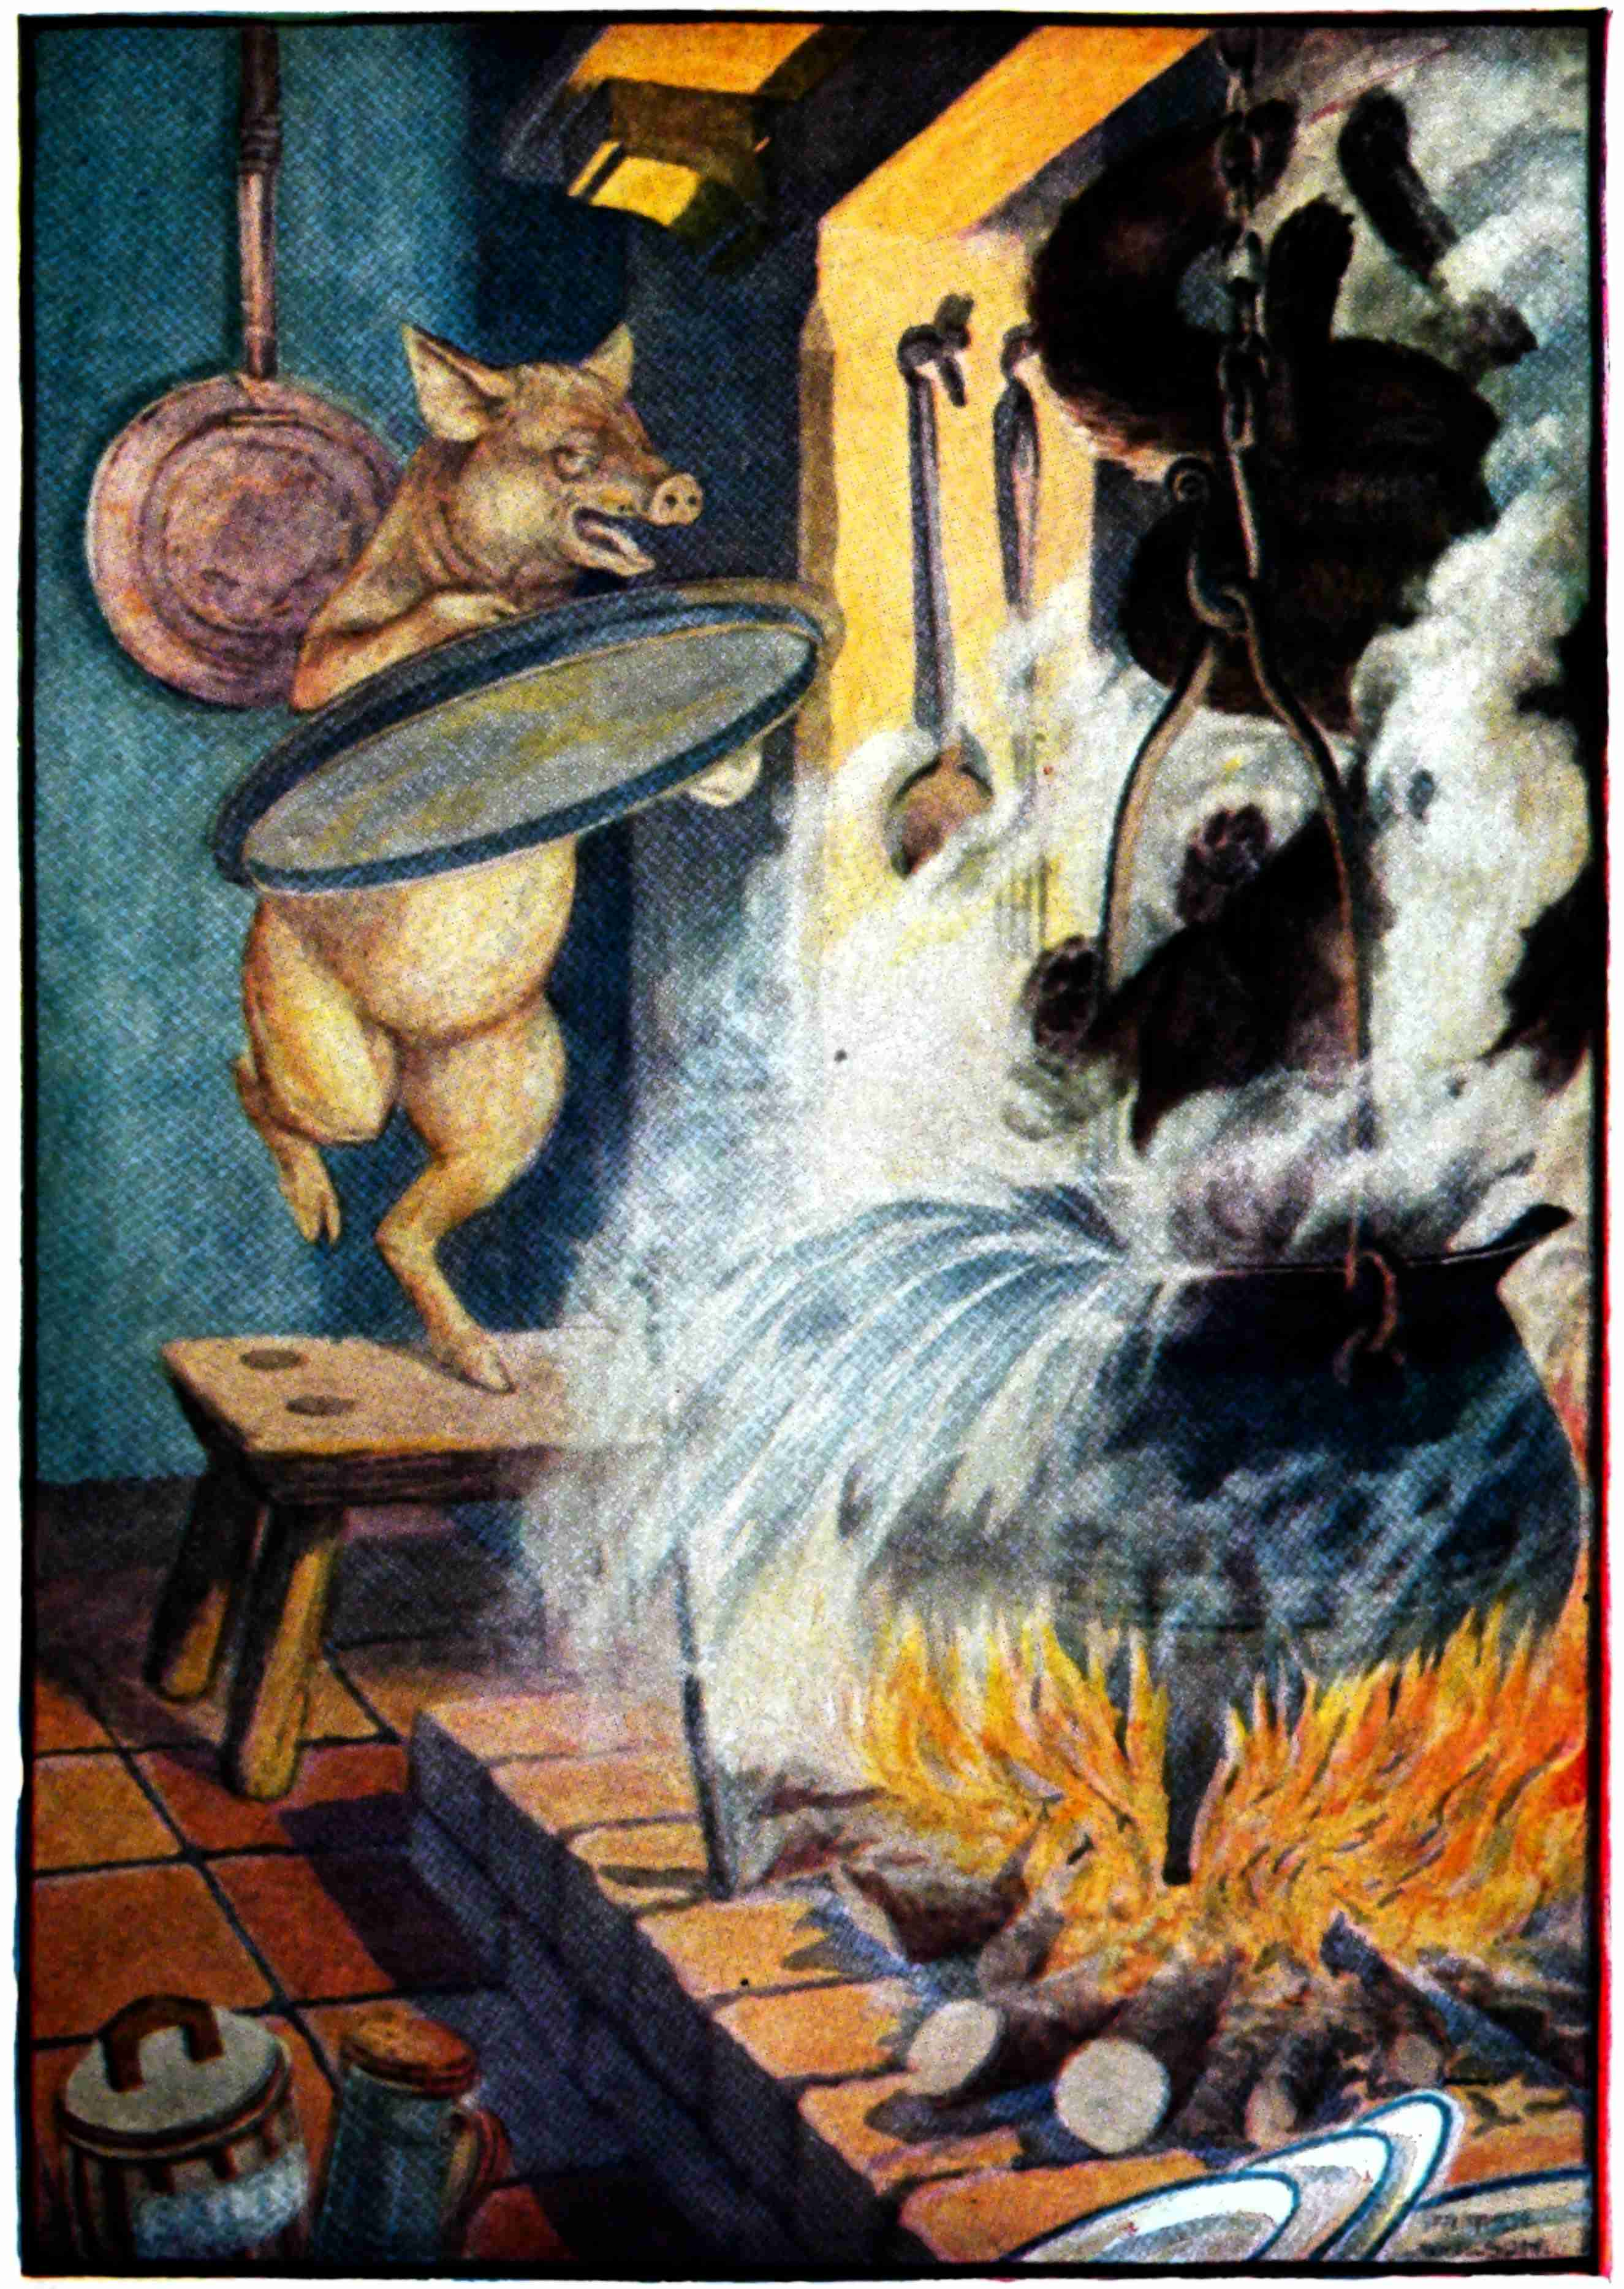
\includegraphics[width=0.98\columnwidth,height=0.99\textheight,keepaspectratio]{pages.jpg/004}
\par\end{center}

\vspace*{\fill}

\clearpage{}

\vspace*{\fill}

\noindent \begin{center}
\includegraphics[width=0.98\columnwidth,height=0.99\textheight,keepaspectratio]{pages.jpg/005}
\par\end{center}

\vspace*{\fill}

\clearpage{}

\vspace*{\fill}

\noindent \begin{center}
\includegraphics[width=0.98\columnwidth,height=0.99\textheight,keepaspectratio]{pages.jpg/006}
\par\end{center}

\vspace*{\fill}

\clearpage{}

\vspace*{\fill}

\noindent \begin{center}
\includegraphics[width=0.98\columnwidth,height=0.99\textheight,keepaspectratio]{pages.jpg/007}
\par\end{center}

\vspace*{\fill}

\clearpage{}

\vspace*{\fill}

\noindent \begin{center}
\includegraphics[width=0.98\columnwidth,height=0.99\textheight,keepaspectratio]{pages.jpg/008}
\par\end{center}

\vspace*{\fill}

\clearpage{}

\vspace*{\fill}

\noindent \begin{center}
\includegraphics[width=0.98\columnwidth,height=0.99\textheight,keepaspectratio]{pages.jpg/009}
\par\end{center}

\vspace*{\fill}

\clearpage{}

\vspace*{\fill}

\noindent \begin{center}
\includegraphics[width=0.98\columnwidth,height=0.99\textheight,keepaspectratio]{pages.jpg/010}
\par\end{center}

\vspace*{\fill}

\clearpage{}

\vspace*{\fill}

\noindent \begin{center}
\includegraphics[width=0.98\columnwidth,height=0.99\textheight,keepaspectratio]{pages.jpg/011}
\par\end{center}

\vspace*{\fill}

\clearpage{}

\vspace*{\fill}

\noindent \begin{center}
\includegraphics[width=0.98\columnwidth,height=0.99\textheight,keepaspectratio]{pages.jpg/012}
\par\end{center}

\vspace*{\fill}

\clearpage{}

\vspace*{\fill}

\noindent \begin{center}
\includegraphics[width=0.98\columnwidth,height=0.99\textheight,keepaspectratio]{pages.jpg/013}
\par\end{center}

\vspace*{\fill}

\clearpage{}

\vspace*{\fill}

\noindent \begin{center}
\includegraphics[width=0.98\columnwidth,height=0.99\textheight,keepaspectratio]{pages.jpg/014}
\par\end{center}

\vspace*{\fill}

\cleardoublepage{}

\chapter{ᎤᏍᏗ ᎦᎵᎩᎾ}

\vspace*{\fill}

\noindent \begin{center}
\includegraphics[width=0.98\columnwidth,height=0.99\textheight,keepaspectratio]{pages.jpg/015}
\par\end{center}

\vspace*{\fill}

\clearpage{}

\vspace*{\fill}

\noindent \begin{center}
\includegraphics[width=0.98\columnwidth,height=0.99\textheight,keepaspectratio]{pages.jpg/016}
\par\end{center}

\vspace*{\fill}

\clearpage{}

\vspace*{\fill}

\noindent \begin{center}
\includegraphics[width=0.98\columnwidth,height=0.99\textheight,keepaspectratio]{pages.jpg/017}
\par\end{center}

\vspace*{\fill}

\clearpage{}

\vspace*{\fill}

\noindent \begin{center}
\includegraphics[width=0.98\columnwidth,height=0.99\textheight,keepaspectratio]{pages.jpg/018}
\par\end{center}

\vspace*{\fill}

\clearpage{}

\vspace*{\fill}

\noindent \begin{center}
\includegraphics[width=0.98\columnwidth,height=0.99\textheight,keepaspectratio]{pages.jpg/019}
\par\end{center}

\vspace*{\fill}

\clearpage{}

\vspace*{\fill}

\noindent \begin{center}
\includegraphics[width=0.98\columnwidth,height=0.99\textheight,keepaspectratio]{pages.jpg/020}
\par\end{center}

\vspace*{\fill}

\clearpage{}

\vspace*{\fill}

\noindent \begin{center}
\includegraphics[width=0.98\columnwidth,height=0.99\textheight,keepaspectratio]{pages.jpg/021}
\par\end{center}

\vspace*{\fill}

\clearpage{}

\vspace*{\fill}

\noindent \begin{center}
\includegraphics[width=0.98\columnwidth,height=0.99\textheight,keepaspectratio]{pages.jpg/022}
\par\end{center}

\vspace*{\fill}

\clearpage{}

\vspace*{\fill}

\noindent \begin{center}
\includegraphics[width=0.98\columnwidth,height=0.99\textheight,keepaspectratio]{pages.jpg/023}
\par\end{center}

\vspace*{\fill}

\clearpage{}

\vspace*{\fill}

\noindent \begin{center}
\includegraphics[width=0.98\columnwidth,height=0.99\textheight,keepaspectratio]{pages.jpg/024}
\par\end{center}

\vspace*{\fill}

\cleardoublepage{}

\chapter{ᏈᏘ ᎠᎴ ᏔᏫᏘ}

\vspace*{\fill}

\noindent \begin{center}
\includegraphics[width=0.98\columnwidth,height=0.99\textheight,keepaspectratio]{pages.jpg/025}
\par\end{center}

\vspace*{\fill}

\clearpage{}

\vspace*{\fill}

\noindent \begin{center}
\includegraphics[width=0.98\columnwidth,height=0.99\textheight,keepaspectratio]{pages.jpg/026}
\par\end{center}

\vspace*{\fill}

\clearpage{}

\vspace*{\fill}

\noindent \begin{center}
\includegraphics[width=0.98\columnwidth,height=0.99\textheight,keepaspectratio]{pages.jpg/027}
\par\end{center}

\vspace*{\fill}

\clearpage{}

\vspace*{\fill}

\noindent \begin{center}
\includegraphics[width=0.98\columnwidth,height=0.99\textheight,keepaspectratio]{pages.jpg/028}
\par\end{center}

\vspace*{\fill}

\clearpage{}

\vspace*{\fill}

\noindent \begin{center}
\includegraphics[width=0.98\columnwidth,height=0.99\textheight,keepaspectratio]{pages.jpg/029}
\par\end{center}

\vspace*{\fill}

\cleardoublepage{}

%redefine Chapter header placement
\titleformat{\chapter}[display]
	{\normalfont\huge\bfseries}
	{\chaptertitlename\ \thechapter}
	{20pt}
	{\Huge}
\titlespacing*{\chapter}{0pt}{50pt}{40pt}

\chapter{ᏣᎳᎩ-ᏲᏁᎦ}

\setlength{\columnsep}{20pt}\setlength{\columnseprule}{.5pt}\begin{multicols}{2}

The following English translations are only approximations of the
Cherokee language dialogue and may be completely different in meaning
in some cases.

\section{ᎦᏁᎳ ᏍᏆᎩ ᏔᎩ}

ᎦᏁᎳ ᏍᏆᎩ ᏔᎩ - Mrs. Squawky Tawky

ᏃᏊᏍ ᏗᏥᏲᏟ, ᏛᏨᏃᏎᎵ ᏥᏔᎦ ᏄᏛᏂᏗ ᎦᏅᏅᎢ ᏧᏂᏗᏫᏍᏗᎢ.

Now y'all children, I will explain for y'all what a chicken does before
crossing a roadway.

ᎠᎬᏱᎢ- ᎣᏍᏓ ᎭᎦᏎᏍᏓ ᎠᎦᏘᏌ ᏗᏜ\ldots{} - First- Watch carefully towards the
right \ldots{}

ᏃᎴ ᎣᏍᏓ ᎭᎦᏎᏍᏓ ᎠᎦᏍᎦᎾ ᏗᏜ\ldots{} - And then watch carefully towards the
left \ldots{}

Ꮓ ᏂᎦᏓ ᏕᏗᏂᏗᏫ ᎤᏟᏍᏓ! - And then we all cross fast!

ᏗᏥᏲᏟ! ᎭᏢ ᎡᏤᏙᎭ? - Y'all children! Where are y'all about?

ᎣᏂᏗᏜ ᎯᏙᎬᎢ, ᎡᏥ! - Behind of where you are standing, mother!

ᎦᏙ ᎡᏣᏛᎦ ᎢᏥᎷᎩ ᎠᎭᏂ? - What did y'all do to just arrive here?

Ꮎ ᎭᏫᏂᏗᏜ ᎦᎶᎯᏍᏙᏗ ᏦᏨᏂᏓ! - That underneath way-point, our staying alive!

ᎲᏂᏓ ᎭᏫᏂᏗᏜ ᎦᎶᎯᏍᏙᏗ ᏣᏓᎦᏎᏍᏙᏗ. - Stay alive, underneath way-point for your
self protection.

\section{ᏧᏟ ᏩᎦᏂ}

ᏧᏟ ᏩᎦᏂ - Fox Fagan

ᏥᏔᎦ ᎨᎵᏍᎩ\ldots{} ᏥᏔᎦ Ꮃ ᎤᎬᏫᏳ\ldots{} ᏥᏔᎦ ᏫᎦᏎ\ldots{} ᏥᏔᎦ\ldots{} ᏥᏔᎦ\ldots{}
ᏥᏔᎦ\ldots{} ᏂᎦᎥ ᏗᎬᏂᏍᏙᏗ - Chicken pie\ldots{} Chicken “la” king/chief\ldots{}
Chicken Fricasse\ldots{} Chicken\ldots{} Chicken\ldots{} Chicken\ldots{}
for any of these recipes.

ᏌᏊ ᎠᎦᏴᎵ ᏂᏗᎬᏂᏗ ᎬᏂᏍᏙᏗ ᏥᏔᎦ - One thousand preparation recipes for chicken.

ᎠᏆᎾᏔ ᎭᏢ ᏌᏊ ᏱᏥᏂᏯ\ldots{} Ꮎ ᏗᎦᎶᎩᏍᎩ ᎤᏬᏗᎨ ᏥᏔᎦ ᎤᎾᏁᏍᏗᎢ - I know where one
I might catch\ldots{} That Farmer Brown, chickens their-flexible-holding-place.

ᎠᏎᏃ ᏏᎸᏍᏓ, ᏥᏓᎢᏅᏓ Ꮎ ᏄᏓᎾᏛᎾ ᎤᎦᏎᏍᏓ ᎩᏟ! - But there is a cause to wait a
minute, I must get rid of that none-thinking watch dog!

\subsection*{(ᏐᎢ ᎪᏪᎵ)}

ᎭᏩ ᏃᏛ! - Alright then!

ᎣᏏᏲ ᎩᎾᎵ, Ꮭ ᎪᎱᏍᏗ ᏱᎦᎮᎳ, ᏞᎦ ᏗᎦᏙᎳ ᏗᏣᎾᏬ! - Hello my friend, Not something
that will bother, I need to use your clothes a while!

ᎯᎠ ᏗᎾᏬ, ᎤᏙᎯᏳ ᎠᏯ ᎤᏠᏯ Ꮎ ᏗᎦᎶᎩᏍᎩ ᎤᏬᏗᎨ. - This clothing, really I same-as
that Farmer Brown.

Ꭾ ᏂᎯ! - Hey you!

ᏝᎨ ᏧᏟ ᏘᎨᎯᏙᏱᎩ ᎥᎿ ᏗᏆᏤᎵ ᏥᏔᎦ? - You are watching for foxes there where
my chickens are or not?

Ꭷ, ᎩᎳᎢᏳᏍᏗ ᏥᎪᏩᏔ ᏧᏟ ᎠᏨᏏᏱᏙᎲᎢ ᎾᎥ ᏅᏲ ᎠᏐᏴᎢ\ldots{} ᏓᏤᏝ ᏃᏊ ᏱᏣᏂᎩᏌ!! - Ka, someone
like that I just saw, a fox snooping around near the rock wall\ldots{}
Now it is better if you really get started!!

ᏥᏌᎹᏓ! ᏍᎩᏛ ᎤᏙᎯᏳ ᏥᏌᎹᏓ!! - Smart! Yeah that's it, I'm very smart!

ᎣᏏᏊ ᏒᎯᏰᏯᏗᏜ ᎢᏥᎨ? ᏙᎯᏊ ᏁᏣᏛᏁᏍᏗ\ldots{} ᎡᎷᏊ ᎠᏋᏌ ᏱᎦᏓᏍᏕᎳᎯᏓ. - It is just a
swell evening ladies? Just peaceful let you all become\ldots{} I am
about to help myself.

\subsection*{(ᏐᎢ ᎪᏪᎵ)}

ᎯᎠᎨᏒ ᎣᏍᏓᎨᏒ Ꮎ ᏫᎧᏎ! - This one is good as that Fricasse!

ᎯᎠᏃ\ldots{} Ꭵ Ꭵ\ldots{} ᎠᏟᎩᏍᎩ ᎡᏙᎯ - And this one\ldots{} uh uh \ldots{}
sleeper walker.

ᎯᎠᎾᏗᏜ\ldots{} ᏥᏔᎦ ᎨᎵᏍᎩ - Towards this\ldots{} chicken pie!

ᎡᏣᎦᏎᏍᏕᏍᏗ ᎢᏥᎨ! ᏱᏬᎦᎶᎯᏍ ᏭᎵᏍᏛᎢ - You all will be being careful ladies!
There is a short drop at the end

Ꭳ, Ꭳ, ᎠᏰᏥᏙᎯ\ldots{} Ꮎ ᏗᎦᎶᎩᏍᎩ ᎤᏬᏗᎨ ᏳᏛᎦᏅ ᏂᎦᏪᏍᎬᎢ, ᎠᏯᏃ ᎠᎩᎵᏬᏨ ᎧᏬᏄ\ldots{}
ᎾᏕ ᏧᏟ! - Oh, oh, waking up walker\ldots{} That Farmer Brown hears her
making a noise, then I am a dead duck\ldots{} I meant to say fox!

ᏓᏂᏥᏃᎨᏎᎵ ᏫᎦᏢᏍᎬ ᎪᎯᏓ - I'll sing her to being asleep for a long time.

“ᎦᏥᏟᎨᎯᏍᏗᎯ ᎤᏍᏗᎢ” - “Rock-a-Bye Baby”

\subsection*{(ᏐᎢ ᎪᏪᎵ)}

ᏥᎪᏫᏘ Ꮓ Ꮎ ᏅᏲ ᎠᏐᏴ\ldots{} I see now that stone fence\ldots{}

ᎭᏩ ᏧᏟ, ᏃᏊᏍ ᏗᎦᎢ, ᎡᏣᏛᏅ ᎠᎴ ᎡᏣᏁᎦᎸᏗ!! - Alright fox, now I'm coming, you
will be hanged and skinned!!

ᎠᏲ! - Ouch!

ᎾᎯᏳᏃ\ldots{} And then\ldots{}

ᏄᏁᎩᎵᏓ ᏂᎦᏛᏁᎭ\ldots{} ᏧᏟ ᏕᎧᏃᎩᏏᎭ ᏥᏔᎦ! - Absurdity this\ldots{} A fox singing
for a chicken!

“ᎦᏥᏟᎨᎯᏍᏗ ᎤᏍᏗᎢ” - “Rock-a-Bye Baby”

Ꭽ! ᎯᎠ ᎠᎬᏱ ᏗᏥᏃᎩᏏᎲ ᏥᏔᎦ ᎬᏂᏍᏙᏓ - Ha! This is first time I ever sang to
a chicken dinner

\subsection*{(ᏐᎢ ᎪᏪᎵ)}

ᏃᏊᏍ ᎠᏯ\ldots{} - Now I\ldots{}

ᏏᎸᏍᏗ ᏌᏊ ᎢᏯᏔᏬᏔᏅᎢ, ᎩᎾᎵ - Wait one minute, my friend

ᏝᏢ ᏱᏥᎪᏫᏔ Ꮎ ᏧᏟ Ꮎ ᏅᏲ ᏣᏐᏯ - I didn't see that fox at that stone fence
of before

ᏅᏲᎩ ᏣᏐᏯ? \ldots ᏂᎪᏫᏘᎲᎾ ᏧᏟ! - Stone fence of before? \-that is (why)
without seeing a fox!

ᏅᏲ ᎠᏔᎴᏒ ᎠᎹᏱ ᏥᎦᏓ\ldots{} ᏄᎳ ᏕᎮᎾ, ᏱᎬᎪᏩᏛᏓ! - Stone hole water-place I
said where\ldots{} Hurry up and go my way, I'm about to show you!

ᎪᎱᏍᏗ ᎾᏆᏍᏓ, ᏕᏥᎵᎡᎾ ᎠᎴ ᎾᏆᏓᎾᏛᎾ - Something either of me, I am deaf or
I am without thinking.

Ꮒ! ᎥᎿᎢ ᏧᏟ! - ᎠᎩᎢ! - Look! Therein is the fox!

ᎭᏢ? - Where?

ᎠᎭᏂ! - Here!

\subsection*{(ᏐᎢ ᎪᏪᎵ)}

ᏧᎻ! - Splash

Ꭷ, ᏥᎯᎱᎸᎦ! - Ka, he is washed up.

Ꭾ! ᎢᏥᏅᎪᎯ ᎦᏅᏛᎢ? - Hey! You all have exited out of the bag?

Ꭾ ᎠᏍᎦᏯ! - Hey man!

ᎦᏙᎤᏍᏗᏃ\ldots - And what thing\ldots{}

ᏧᏟ ᏂᎬᎵᏍᏓᏁᎭ! - Fox I am happening to you!

Ꮭ! ᎠᏯ ᏗᏥᎶᎩᏍᎩ ᎤᏬᏗᎨᎢ - ᏍᎩᎪᎲᏛ! - No! I am Farmer Brown - you see me!

ᏙᏛ, ᎠᏎᏃ Ꮭ ᎴᎯᏳ ᏱᏂᏓᏙᎢ! - Sure, but not ever having a tail!

\subsection*{(ᏐᎢ ᎪᏪᎵ)}

Ꭾ? ᏣᏙᏓᏍ ᎤᏅᏔ ᏣᏅᎪᏨ? - Hey! Does your father know you are out?

ᎤᏅᏔᏛ! - He does!

ᎥᎥ! - uh uh

ᎥᏍᎩᎾ ᎠᎩᏙᏓ! - That is my dad!

ᎬᏅᎨᏒ ᎠᏓᏅᏖ, Ꮭ ᎠᏯ ᎨᏒ Ꮎ ᏗᎦᎶᎩᏍᎩ ᎤᏬᏗᎨᎢ. - Obviously he is thinking, I am
not that Farmer Brown

ᏕᎯᏴᎯᏊ! ᎬᎦᏘᏴᎢ! - Come in! I was expecting you!

ᎣᏏᏛᏃ ᎥᏍᎩᎾ ᎣᏂᏱᎩ ᎥᎩᏲᏍᏓᏁᎲᎢ, ᎠᏆᏓᎦᏍᎦᏃ . . . ᎠᏎᏃ ᏝᎨᏒ ᏥᏔᎦᎨᏒ!! - I hope that
is the last interruption. I am getting fed up, but not with chicken!

ᎮᎦᏍᏓᎭ ᎢᏥᎨᏳᏣ, Ꮭ ᏯᏩᏢᏓᎾᏁᎭ ᏂᎦᏓ ᎨᏒᎢ, \ldots - I am sorry girls but I don't
have time for all of you, so \ldots{}

\subsection*{(ᏐᎢ ᎪᏪᎵ)}

\ldots ᏓᏥᎾᏫᏛ, ᎠᎴ ᏫᏓᏤᏢ ᏩᎾ ᎨᏎᏍᏗ - The biggest I am taking away, and
you better be tender!

Ꭳ, Ꭳ, ᎯᎠ ᎨᏒ ᎠᏛᏅᏍᏗ ᎤᏝᏫᏗᏍᏗᎢ - Oh oh - this one is ready to take off

ᎦᏍ! ᏙᏳ ᎦᎸᎳᏗ ᎦᏃᎯᎵᏙᎯ - Gosh! Truly an up high flyer.

ᎢᎢᎢᎢᏲᏫᎢᎢ - Eeeeeyyoow

ᏧᎻ! - Splash!

ᎧᏩᎧ! - Kawack!

\subsection*{(ᏐᎢ ᎪᏪᎵ)}

ᎠᏎᏛᎲ, Ꮭ ᎦᏥᏂᏯ ᏧᏟ. - I guess I won't catch a fox.

ᎠᏲ! - Ouch!

Ꭳ, ᏂᎭᏕᏃᎴ\ldots{} ᏝᎨ Ꮟ ᎯᏂᏴᏛᏱᎩ Ꮎ ᏧᏟ? - Oh! it is you again - You catch
that fox yet or not?

ᎠᏎᏛᎲ Ꮭ ᎣᏍᏓ ᏗᏥᎴᎾᎯᏓᏱᎩ ᎠᏯ ᏱᎩ - I guess I was not cut out to be a fox
hound

Ꭷ, ᏏᎸᏍᏗ ᏌᏊ ᎢᏳᏩᎦᏓ ᏛᎬᎵᏍᎪᎵᏓᏁᎵ - Ka, yet a moment, I am going to give
you one more chance!

\subsection*{(ᏐᎢ ᎪᏪᎵ)}

ᎯᎪᏫᏘᎭᏍ Ꮎ ᎦᏚ ᎧᎵᏦᏛ ᏧᎩᎳ ᏥᏔᎩ, ᎯᏯᎦ ᎯᎠ ᎦᏂᏙᏗ, ᎠᎴ ᎬᏂᎨᏒ ᏱᏂᏥᏴᎦ Ꮎ ᏧᏟ. - Do you
see that chicken up there on the roof, put it in this bag, and in
view I will make the fox!

Ꮵ, ᏩᏙ! - Gee, thanks!

ᎠᎯᏓ ᎯᎢᎾ, ᎾᏊ ᏥᏌᎹᏓ ᎩᏟ - This is easy, now I am a smart dog

ᎬᏂᏯ! - I got you!

ᎠᎧ! - Awk

ᎯᏂᏯᏍ, ᎭᏗ? - You got it, you just said?

ᎤᏙᏳᏛ! - Most truly!

Ꭷ, ᎭᏩ! ᏘᏲᎯᏗᎾ! - Ka, alright! You will give it!

ᎠᎭᏂ ᏓᏳᏍᏗᏓ! - Here it comes!

ᏞᏂᎧ! - Clank!

\subsection*{(ᏐᎢ ᎪᏪᎵ)}

Ꭽ! ᏙᏳ ᏭᎨᏗᏴ ᎡᎶ ᎡᎯ ᏥᏔᎦ! - Hah! Truly most heavy chicken in the world!

ᎭᏓᎾᏘᏓ\ldots{} ᏣᏛᏍᏔᏅ ᏍᎩᎪᏩᏛᏗ Ꮎ ᏧᏟ - Remember\ldots{} You promised me for
you to show me the fox

ᎠᎭᏂ ᏣᎵᎶᏥᏓ!! - Here you lacking one!

ᎠᏊᏌ ᎦᏓᎵᏍᏓᏅᎢ! - Myself doggoned!

ᏧᏟ! ᏥᏂᎭᏛᎦ!! Ꭾ! Ꭾ! - Fox! Again you did it!! Heh! Heh!

\subsection*{(ᏐᎢ ᎪᏪᎵ)}

ᏛᎻ! ᏛᎻ! ᏏᎸᏍᏗ\ldots{} ᎦᏣᎸᏅ\ldots{} ᎦᏚᏅ\ldots{} ᎠᎵᏓᏅᎢ ᎥᏍᎩ\ldots{} ᎠᎵᏓᏅᎢ!
- Tum! Tum! Just a minute\ldots{} Fried\ldots{} Roasted\ldots{} Boiled\ldots{}
Boiled!

ᏏᎸᏍᏓ ᎠᎬᏱ ᎦᏲᏟ ᏗᏓᎵᏥᏍᏗᏍᎩ ᏃᎴ ᎦᏲᏟ ᏆᏍᎵ\ldots{} - Just a minute first a small
amount of carrots then a small amount of parsley\ldots{}

ᏃᏊᏛᎨᏒ - Ꮎ ᏥᏍᏆ!! - Truly now being - The bird!

ᎠᎧ! - Awk!

ᏙᏳ ᎤᏄᏗᏱ, ᎠᏎᏃ\ldots{} ᏥᏔᎦ!! - Very tough, but\ldots{} it is chicken!

ᎠᎵᏍᏆᏓ - End

\section{ᎤᏍᏗ ᎦᎵᎩᎾ}

ᎤᏍᏗ ᎦᎵᎩᎾ - Little Buck

ᎠᏙᎯᏍᏗ ᎦᏛᎩᏍᎦ! - His yell I hear!

ᏙᏳ ᎤᎵᎮᎵᏍᏓ, ᏙᎨᎤᏍᏗ ᏂᎦᎵᏍᏗᎭ? - He sure is excited, wonder what is up?

Ꭷ! ᎦᏙᎦᎵᏍᏗᎭ, ᎤᏍᏗ ᎦᎵᎩᎾ? - Gosh! What is wrong buck?

ᏈᏂᏙ! ᎢᏂᏃᎭᎴᎦ! Pinto! We are going hunting!

ᎠᏎᏃ Ꮭ ᏣᏓᎾᏖ ᎢᏳᏍᏗ! - But not the way you think!

ᏝᏃ ᎦᎵᏣᏗ ᎠᎴ ᏗᎦᏟᏓ ᏃᎴ ᏅᏱ ᎤᏕᎩ ᏃᎴ ᎦᎶᏪ, ᎪᎯᏊ ᏄᏍᏗᏓᏅᎢ. - No more bow and arrows
or slingshots or rifles, we are going modern!

ᎠᏓᏟᎶᏍᏗᏍᎩ ᏓᏅᎾᏛᏂ! - We are using a camera!

\subsection*{(ᏐᎢ ᎪᏪᎵ)}

ᏙᏳᏛ ᎠᏓᏟᎶᏍᏗᏍᎩ ᎤᎪᏓ ᎠᎯᏓ ᎥᎿ ᎢᎾᎨ ᎠᏁᎯ ᎠᏎᏃ ᎨᏒ ᎦᏟᏓ ᎠᎴ ᏗᎦᏟᏓ! - You have got
to admit a camera is a lot easier on animals than a bow and arrow!

ᏂᏯ ᏥᎦᏗ\ldots{} ᎠᏂᎸᏉᏗᎭ! - See what I mean\ldots{} They love it!

ᏟᎧ! - Click!

ᏃᏊ\ldots{} ᏣᏰᏣ! - Now\ldots{} Smile!

ᏃᏊᏍ ᏄᏓᎴ ᏄᏍᏗᏓᎾ, ᏈᏂᏙ\ldots{} ᎢᎾᎨ ᎠᏁᎯ ᏃᏊ ᏗᎨᎩᏂᎸᏉᏓ! - Things are different
now, Pinto\ldots{} The animals all love us!

ᎠᏎᏃ ᎯᎠ ᎠᎯᏗᏊ\ldots{} ᎤᎪᏓ ᏧᎵᏤᎩ ᏗᎩᏂᏟᎶᏍᏓ! - But this stuff is too tame\ldots{}
What we need are some unusual shots!

Ꮒ! ᏧᏙᏓᎸᎢ\ldots{} ᎠᏬᎭᎵ ᎤᏩᏁᏍᎬᎲᎢ - Look! up there on the cliff \ldots{}
An eagle's nest!

Ꮒ , ᏄᎵᏍᏗᏓ ᎤᏂᏥ ᎠᏬᎭᎵ - And there goes the mother eagle.

\subsection*{(ᏐᎢ ᎪᏪᎵ)}

ᏄᎳ ᏈᏂᏙ! ᎦᏚ ᏫᏓᏂᎸᏍᏓᏂ, ᏗᏟᎶᏍᏙᏗ ᎾᎥᏂᎨᏍᏗ ᎠᏬᎭᎵ ᏧᏪᏥ. - Come on Pinto! we are
going to the top for some eagle-egg close-ups!

ᏙᏳᎧ\ldots{} ᏂᏚᏬᏚᎯ! ᎤᏟᏍᏓᏍ ᏗᎩᎶᏫᏍᏓᏏ, ᏏᎸᏍᏓ ᏄᎷᏨᎾ ᎤᏂᏥ ᎠᏬᎭᎵ. - Boy o' boy\ldots{}
What beauties! We gotta work fast before mother eagle gets back

ᏏᎸᏍᏓ ᎠᎬᏱ ᏗᏂᎧᏁᎦ ᏍᏕᏱᏛ ᎥᎿ ᎯᏂᏓᏛᎢ\ldots{} ᏐᎢᏃ ᎦᎸᏪᏍᏙᏗ ᎠᏩᏓᏠᏍᏗᎢ - First, we
tie this rope to your tail\ldots{} and the other end around my waist

Ꮓ, ᏙᎢ ᎡᎳᏗᏜ - Then I let myself down easy

ᏞᏍᏗ ᏨᏨᎨᏫᏏ\ldots{} ‘ᎭᏏᏄᎦ’ ᎠᏰᎸᏓ Ꮎ ‘ᎡᎳᏗᏜ’\ldots{} ᎠᎴ ‘ᎭᏂᎩ’ Ꮎ ᎠᏰᎸᏓ ‘ᎠᏌᎵᏙᏗ’!
- Now remember\ldots{} “Back up” means “down”\ldots{} and “giddap” means
“up”!

‘ᎭᏏᏄᎦ’ Ꮎ ᎠᏰᎸᏓ ‘ᎠᏌᎵᏙᏗ’\ldots{} Ꮟ, ᎾᏕ ‘ᎡᎳᏗᏜ’ Ꮎ ᎠᏰᎸᏓ ‘ᎭᏂᎦ’ Ꮭ\ldots{} ᎠᏌᎵᏙᏗ\ldots{}
ᎡᎳ\ldots{} - Back up means up\ldots{} I mean down and down means giddap\ldots{}
no\ldots{} up\ldots{} dow\ldots{}

ᎭᏩ\ldots{} ᎭᏏᏄᎦ! ᎯᏒᎵᏚᎦ, ᎯᏒᎵᏛᎦ! ᏏᎸᏍᏗ ᏍᏗᏊ! - Ok\ldots{} Back up! Up up!
A little more!

\subsection*{(ᏐᎢ ᎪᏪᎵ)}

ᎭᎴᏫᏍᏓ! ᏙᏳᎧ! ᏗᏟᎶᏍᏙᏗ\ldots{} ᎡᎵᏍᏗ ᎪᎱᏍᏗ ᏱᎦᏓᏌᎾ! - Whoa! Boy o' boy! What
a shot\ldots{} I should win something with this!

ᎪᎱᏍᏗ ᏛᎩᏲᏎᎵ ᎾᏆᎵᏍᏓᏁᎭ ᎯᎠ! - Feels as if I am going to lose something
with this!

ᏥᏥᏥᏥᏥᏥᏥ - zzzzzzz

Ꭳ\ldots{} Ꭳ! ᎠᏛᏩᎦᏘᎯᏙᎯ - Oh\ldots{} Oh! A visitor

ᎭᏛᏓᏍᏓ! ᏝᎨ ᏱᏍᎩᎪᏫᏘ ᏓᎩᎶᏫᏍᏓᏁᎲᎢ? ᎭᏂᎩ!! - Listen! Can not you see I am busy?
Scram!!

ᎭᏩ\ldots{} ᏨᏌᏊ!! - All right\ldots{} You asked for it!

ᏩᎧ! - Whack!

\subsection*{(ᏐᎢ ᎪᏪᎵ)}

Ꭴ! - Ooph!

Ꭾ, Ꮭ ᏱᎦᏛᏛᎦ ᏣᏛᏅ, ‘ᎭᏂᎩ!’ - Hey! I didn't hear you say giddap!

Ꮭ ᏱᏂᏥᏫ!! - I did not say it!!

ᏃᏊᏛ\ldots{} ᎦᏛᏅᏖᎳ! ᏞᏍᏗ ᏨᎠᏖᎸᎾ, ᎬᏂᎩᎳ, ‘ᎭᏂᎩ’ ᏯᏆᏛᎾ! - Now\ldots{} remember
do not move a muscle unless I say giddap!

ᎡᎷᏊᏍ Ꮭ ᎪᎱᏍᏗ ᏱᎦᎩᎲᎾ\ldots{} ᏝᏍᏊ ᎦᏙ ᏳᏖᎸᎾ! - Betcha nothing could move
me\ldots{} not even an earthquake!

ᎭᏩ\ldots{} ᎭᎦᏙᏍᏓ ᏥᏍᏆ\ldots{} - okay\ldots{} Now watch the bird\ldots{}

ᎦᏙᎤᏍᏗ ᏥᏍᏆ? - What bird?

\subsection*{(ᏐᎢ ᎪᏪᎵ)}

Ꭷ! Ꮎ ᏧᏪᏥ ᎠᎾᎴᏂ ᏓᏂᏯᎢᏍᎬᎢ! - Ka! The eggs are starting to hatch!

ᎡᏥ!! - Mother!!

Ꮭ ᎬᏥ ᏱᎩ - I am not your mother

ᎠᏎᏃ! ᏃᏛ ᏓᏳᏍᏗᏓ! - But! Here she comes now!

ᏍᎩᏕᎳ! ᏈᏂᏙ!! ᏍᎩᏌᎸᏛᎦ — ᏄᎳ! - Help! Pinto!! Pull me up — Hurry!

ᏍᎩᏕᎳ! - Help!

ᎠᏲ! - Ouch!

ᏍᎩᏌᎳᏛᎦ! - Pull me up!

ᏄᎳ! - Hurry!

ᎠᏲ! - Ouch!

ᏄᎾᏍᏛ ᏂᎦᏓ ᏄᎾᏓᏅᏛᎾ ᏗᎦᎾᏢᏓ! - Of all the dumb animals!

ᎦᏙᎲ ᏂᎦᏌᎸᏛᏅᎾ? - Why did not you pull me up?

Ꮭ ‘ᎭᏂᎩ’ ᏱᏍᏉᏏ! - You did not say giddap!

Ꭷ, - ᏙᏳᏛᏃ, ‘ᎭᏂᎩ’! - Ka,- you better start giddapin' rite now!

ᎦᏙᏃ ᏂᎦᏛᎦ? - Now what did I do?

\subsection*{(ᏐᎢ ᎪᏪᎵ)}

Ꭾ! ᏏᎸᏍᏓ ᏞᎦ ᎯᎦᏘᏯ ᎦᎵᎩᏂ ᎦᏙᎤᏍᏗ Ꮎ ᎾᎥ ᏧᏍᏓᎪᎸᎢ? - Hey! Wait a minute buck
what is that over there by the cave?

ᏈᏂᏙ! ᎠᏂᏓ ᏢᏓᏥ - Pinto! It's a mountain lion cub

Ꭷ! ᎤᏙᎯᏳᎭ ᏗᏟᎶᏍᏓᏅ ᎯᎠ ᎨᏎᏍᏗ! - Ka! What a picture that will make!

ᏣᏅᎨᏍᏗ! ᎤᏙᎯᏳ ᎩᏂᏍᎪᎵᏓᏁᎭ! ᎭᏓᎾᏖᎳ! “ᎤᏍᏗ ᎦᎵᎩᎾ” ᎡᎶᎯ ᏗᎦᏃᏣᎵ ᏗᎦᎾᏢᏗ ᏗᏟᎶᏍᏗᏍᎩ. -
Hurry up! This is our big chance! Imagine it! “Little Buck” World
famous animal photographer.

ᎾᎥ ᏫᎩᏂᎷᏣ ᏱᏂᏩᏛᏓ! - When we get close we will sneak up on him!

ᏁᏙᎲᎾ! - Gone!

\subsection*{(ᏐᎢ ᎪᏪᎵ)}

Ꮒ! ᏧᎳᏏᏅ ᏚᏙᎮᎳ ᏧᏍᏓᎪᎸᏗᏜ - Look! His tracks lead into the cave

ᎭᏛᏓᏍᏓ! Ꮟ ᏌᏊᎢᏳᏩᎦᏓ ᏛᎬᎵᏍᎪᎵᏓᏁᎵ!! - Now listen! I am going to give you
one more chance!!

ᎠᎬᏱ, ᏓᏥᎧᏂ ᎯᎠ ᏗᏓᏟᎶᏍᏗᏍᎩ – ᏂᎭᏃ, ᎯᎠ ᏥᏄᏍᏗ ᏣᏐᏅᏙᏗ ᎨᏎᏍᏗ - First, I will prop
this camera up – then all you have to do is push the little gadget

ᎠᏎᎾ ᎮᏍᏗ ᏨᎭᏒᏂᎳ ᎬᏂᎩᎳ Ꮎ ᎠᏂᏓ ᏢᏓᏥ ᏥᏅᎪᏍᏓᏅᎢ - Ꮓ ᎭᎴᎾ ᏕᎭᏟᎶᏍᏗᎲᎢ – ᏞᏍᏗ ᏨᎭᎴᏫᏍᏓᏂ
- But do not touch it until I chase the little cub out - then start
snapping – and do not stop!!

ᎮᏍᏗ ᏯᏓᎾᏖᎸᏍᎨᏍᏗ ᎦᎵᎩᎾ! Ꮭ ᎡᏍᎦ ᏱᏂᏗᎬᏛᏁᏎᎳ ᎯᎠ. - Don't worry buck! I won't
let you down this time.

ᏕᎮᎾ - ᏪᏌ - ᏪᏌ! ᏘᏅᎪᎢ ᎠᎴ ᏕᏣᏟᎶᏍᏓ! - Here - Cat - Cat! Come out and get
your picture took!

\subsection*{(ᏐᎢ ᎪᏪᎵ)}

ᏗᎭᎳᏓ ᏂᎦᏩ! - Roar!

ᎦᎵᎩᎾ ᎡᎵᏍᏓ ᎦᏂᏯ! - Sounds as if Buck's got him!

ᎣᏍᏓ ᏕᎭᏟᎶᏍᏓ– ᎦᎵᎩᎾ! - Swell shot– Buck!

Ꮟ! - Hold it!

ᏍᎩᏍᏕᎳ! - Help!

ᏣᏰᏣ! - Smile!

Ꭾ ᎦᎵᎩᎾ! ᎡᎷᏊᏍ ᎮᎵᎠ ᏂᎦᎢ? - Hey Buck! Don't you think that is enough?

ᎧᎪ–ᎠᏯᏍ, ᏂᎯᎨ! - Who– me or you?

\subsection*{(ᏐᎢ ᎪᏪᎵ)}

ᏩᎧ! - Whack!

ᎣᏍᏓ! ᎦᎵᎩᎾ, ᎠᏎᏍᏊ ᏕᎦᏟᎶᏍᏓ ᏍᏊ - Great! Buck, I got that one too

Ꮭ ᏱᎪᎵᎦ ᎦᏙᏃ ᎦᎵᎩᎾ ᎥᏍᎩᎾ ᏧᎵᏍᏈᏍᏗ ᏗᏟᎶᏍᏓᏅᎢ - I just can't understand why
Buck wanted to get into all those pictures

Ᏻ-Ꮁ- ᎦᎵᎩᎾ! ᎭᏢ ᎮᏙᎭ? - Yoo - Hoo - Buck! Where are you?

ᎠᎭᏂ, ᏈᏂᏙ-! - Right here, Pinto-!

ᎦᎵᎩᎾ, ᎣᏍᏓ ᎾᏛᎦ- ᏂᎦᏓ ᏥᎩᏐᎭᏂ! - Buck, you are a success- I got everything!

ᎥᏍᎨ ᎮᎵᏍᎦ! - That's what you think!

ᏛᎮᎾ, ᏈᏂᏙ, ᏗᏂᎬᏟᎶᏍᏓᎾᏊ! - Come here again, Pinto!! I am just going to
take your picture!

Ꮭ, ᎡᎷᏊ! Ꮭ ᎣᏏᏊ ᏱᏗᏍᎩᏟᎶᏍᏓ ᎢᎦᎥ ᏱᏓᏬᏘᏌ. - No, enough! I do not photograph
very well with lumps!

\section{ᏈᏘ ᎠᎴ ᏔᏫᏘ}

ᏈᏘ ᎠᎴ ᏔᏫᏘ - Pete and Tweet

ᎠᎩᏙᎦᏏ ᎠᎩᏰᏍᏗᎢ- ᎤᏖᏓ ᎦᎵᏍᎩᏍᎬᎢ! - Ho Hum – I sure hate to wake up- What
a swell dream!

ᏈᏘ ᏗᏥᎧᏁᎲᎢ, ᏧᏬᏰᎾ ᎠᎴ ᏚᎳᏏᏛᎢ \ldots{} - I had Pete tied hand and foot–

ᎾᏆᏛᏅᏒᎢ- ᎦᏙᎲᏃ! ᏃᎴ ᏥᏍᏆ ᎤᏂᎩᏍᏓ ᏌᎾᎴ ᎠᎩᏍᏗ! - And just as I was- And phooey!
Bird seed again for morning food!

Ꮎ ᎾᎩᎸᏆᏛᎾ ᎠᎩᏗ ᎾᎪᎯᎸ ᎤᎪᏓ ᎡᎳᏗᎯᏯ ᎾᏭᏁ ᎠᏎᏃ ᎠᏍᎪᏯ. - Eating that junk day after
day has got me feeling lower than a worm.

\subsection*{(ᏐᎢ ᎪᏪᎵ)}

ᎥᏍᎩᎾ! ᏍᎪᏯ!! Ꮎ ᎠᏂᏥᏍᏆ ᏱᏓᏂᏰᎠ, ᎠᏯᏃᏱᎩ? - That's it! A worm!! If other bird
clan eat them, why not I?

ᎠᏎᏃ ᎠᎬᏱ- ᏥᎶᏎᏍᏗ Ꮎ ᏈᏘ! ᎣᏏᏃ Ꮟ ᏥᎦᏟᎭ. - But first- I have got to get by
Pete! Thank goodness he is asleep!

ᎪᎯᏓ ᎠᎦᏝᏫᏛᎲᎢ, ᏗᎦᏎᏍᏓᎾ! - I have not flown for so long, I better take
the safe way down!

ᎣᏏ ᎨᏎᏍᏗ ᏛᏥᎷᏒᎢ- ᏏᎸᏍᏓ ᎪᎱᏍᏗ ᏱᏄᎵᏍᏓᏂ. - I only hope it will be a safe way
up- Just in case.

Ꮭ ᎴᎯᏳ ᏈᏘ ᎠᎩᏂᏴᏓ ᏱᎩ, ᎠᏎᏃ ᎠᎬᏱ ᏂᎦᎵᏍᏓᏂᏙᎰᎢ. - Pete has never caught me yet,
but there's always a first time!

ᏙᏳ Ꮭ ᏯᎵᏍᎪᏂᏍᎦ-ᏔᏫᏘ! - And you are not kidding-Tweet!

\subsection*{(ᏐᎢ ᎪᏪᎵ)}

ᏞᎦ ᎤᏬᎵᏓ ᏩᏰᎸᎾ ᏏᎸᏍᏓ ᏱᏥᏱᏅᏓ! - I will let him have a little fun before
I nab him!

ᏃᏊ ᏍᎪᏯ ᏙᏳᎢ, ᎦᏳᎳ ᏥᎩᎠ— ᎠᎩ ᏌᏊ! - Now for a worm Boy! I can taste him
now— There is one!

ᏥᏍᏆ! - Bird!

ᏛᎮᎾ! ᎩᎾᎵ– ᎬᏯᏒᏰᏍᏓᏅᎢ ᎥᎿ ᏌᎪᏂᎨ ᎠᏖᎵᏙᎯ!! - Come back here! My friend– I
have got a place for you on a blue plate special!!

ᏕᎭᏓᏅᏗᏍᏓᏂᏙᎲ Ꮎ ᏡᎬᎢ Ꮭ ᏗᏣᏓᏍᏕᎸ ᏣᏂᏱᏍᎬ ᏫᏓᏤᏢ ᏍᎪᏱ ᏗᎦᏂᏱᏍᎩ ᎡᎶᎯ ᎡᎯ. - Ducking
around a tree is not going to save you from the best worm catcher
in the world.

ᎠᎭ! ᎬᏂᏯ! - Aha! Got you!

ᏄᎳ! ᎮᏍᏗ ᏯᏕᎵᎰᏍᎨᏍᏗ ᏂᎯ ᎠᎴ ᎠᏯ Ꮲ ᎢᏁᎦ! - Hurry up! Don't be shy, you and
I are going somewhere!

\subsection*{(ᏐᎢ ᎪᏪᎵ)}

Ꭽ, Ꮒ!! - Ha, Look!!

Ꭳ\ldots{} ‘ᏏᏲ! - Oh\ldots{} Hello!

ᎠᎴ ᎦᏂᎩᎠ! - And goodby!

ᎬᎾᎨ ᏲᎾ ᎢᎾᎨᎢ! ᎠᏴ ᏥᎯᎷᎩ! - Black bears in the woods! I'm coming!

ᎠᎭᏂ ᎠᏆᏗᏍᎦᏞᏍᏗ, ᎠᏂᎩᏍᎬ ᏱᎪᎯᏓ- ᏙᏳᎧ ᎨᎭ!- ᏍᎪᏯ ᏥᎨ ᎠᎴ ᏈᏘ ᎠᎩᎨ- ᏃᎴ Ꮎ ᏍᎪᏯ ᎩᎶ ᎠᎨ!
- I will duck in this can till he goes, what a life!- Me after a worm
and Pete after me- and the worm after somebody else!

ᎠᏎᏃ Ꮭ ᏫᎦᏥᎷᎩ ᏍᎪᏯ ᏥᏘᏁᎲᎾ! - But I can not go back without a worm!

ᎠᎴᏃ ᎠᎭᏂ ᏪᏊ ᎡᎯ ᎥᎿ ᎡᎶᎯ! - And here is the biggest one in the whole world!

ᎬᏂᏯ ᏃᏊᏛ ᎠᎬᏱ ᏍᎪᏯ - Caught you, Now the first worm

ᎯᎠᏃ ᏥᏚᎢᏒ ᎠᎹ- ᏃᏊᏛ- ᏱᎬᏍᏕᎳ ᎠᎩᎯᏍᏗᎢ! - And this I turn the water on - Truly
now- I will help you wash it down!

\subsection*{(ᏐᎢ ᎪᏪᎵ)}

ᎦᎵᏦᎯᏓ ᎤᎵᏍᏓᏁᎭ! - He is sure fattening up!

ᎪᎱᏍᏗ ᎦᏕᎶᎣᏍᎬᎢ - Ꮒ ᏪᏌ! - I was noticing something - you cat!

ᏕᎮᎾ! ᏂᎯ ᎤᎩᏓᎵ ᎠᎹ ᎠᏟᏍᏛ! - Come towards me! You feathered water bottle!

ᎦᏎᎦᏍᏙᏓ Ꮎ ᏪᏌ ᏄᏂᎸᏉᏓ ᎠᎹ— ᏥᎬᏍᏙᏓ ᏗᏓᏩᎵᏔᏚᎦ - Lucky for me cats hate water
— He sure got a mouthful when he jumped on me

ᏍᎩᏕᎳ! ᏥᎬᎦ - Help! I am drowning

ᎾᎪᎯᎸᏃ, ᏥᏚᏍᎨᏍᏗ ᎠᎩᎩᏍᏗ ᏂᎦᏓ ᏥᏍᏊ ᎤᏂᎩᏍᏗ ᎠᎴ ᎠᏆᏓᎾᏓ ᎨᏎᏍᏗ ᏥᏥᏍᏆ- ᎤᏙᎯᏳᎢ!! - And
from now on I promise to eat all my bird seed and be a good bird-
so truly!!

\setlength{\columnsep}{10pt}\end{multicols}\setlength{\columnseprule}{0pt}

\cleardoublepage{}

\end{sloppy}
\end{document}
